% Creating a simple Title Page in Beamer
\documentclass[aspectratio=169]{beamer}
\usepackage{tikz}
\usepackage{tikz-uml}
\usetikzlibrary{shapes}
\usetikzlibrary{arrows}      % use arrow with 90°
\usetikzlibrary{arrows.meta}      % use arrow with 90°
\usetikzlibrary{calc}        % compute midpoint $(A)!0.5!(b)$
\usetikzlibrary{fit}        % fit several nodes
\usetikzlibrary{backgrounds}        % fit several nodes
\usetikzlibrary{positioning}  % of left = of {1cm} NODE
\usetikzlibrary{automata} % draw finite automata
\usetikzlibrary{decorations.markings}
\usetikzlibrary{decorations.pathreplacing} %%curly braces
\usetikzlibrary{decorations.pathmorphing} %% snake, saw
\usetikzlibrary{decorations} %%curly braces
\usetikzlibrary{quotes} %%curly braces
\usetikzlibrary{intersections} % intersections
\usetikzlibrary{patterns}      % fill nodes with pattersn
\usetikzlibrary{tikzmark}      % fill nodes with pattersn

\usepackage{media9}
\usepackage{hyperref}
\usepackage{fancyvrb}
\usepackage{graphicx} % Required to include images
\usepackage{inconsolata}
\usepackage{listings}
\usepackage{balance}
\usepackage{booktabs}
\usepackage[cal=boondox]{mathalfa}
\usepackage[english]{babel}
\usepackage{amssymb}% math symbols as mathbb, \mathsf{d}
\usepackage{amsmath}
\usepackage{amsthm}
\usepackage{mathrsfs}
\usepackage{siunitx} %units
\usepackage{enumerate}
\usepackage{graphicx}
\usepackage{soul}
\usepackage{tabularx}
\usepackage{siunitx}
\usepackage{array}
\normalfont%
\usepackage[T1]{fontenc}
\usepackage{textcomp}
\usepackage{tikz}
\usetikzlibrary{patterns}
\usepackage[utf8]{inputenc}
\usepackage{tikz-cd} % commutative diagrams with tikz
\usepackage[ruled,vlined,linesnumbered]{algorithm2e}
\SetKw{KwTo}{To}
\SetKwRepeat{Do}{do}{while}
\usepackage{caption}
\usepackage{subcaption}

\def\WP{{\mathit{VP}}}
\def\d{\mathsf{d}}
\def\pathv{\mathbf{p}}
\def\path{p}
\def\Rn{\mathbb{R}^n}
\def\R{\mathbb{R}}
\def\Lcal{\mathcal{L}}
\def\Lcalsharp{\mathcal{L}^\#}
\def\Fcal{\mathcal{F}}
\def\Gcal{\mathcal{G}}
\def\Acal{\mathcal{A}}
\def\Mcal{\mathcal{M}}
\def\Ocal{\mathcal{O}}
\def\Ocalfree{\mathcal{O}_{\text{free}}}
\def\Sob{\mathbb{W}^{k,2}}
\def\hatL{\hat{L}}
\def\sinv{s^{-1}}

\newcommand\diff[2]{\frac{\d #1}{\d #2}}
\newcommand\diffp[2]{\frac{\partial{} #1}{\partial{} #2}}
\newcommand\diffk[3]{\frac{\d^{#3} #1}{\d #2^{#3}}}

\def\Fqi{F\big(\qv_i, \dot{\qv}_i,\ddot{\qv}_i\big)}
\def\Gci{G_i\big(\qvnom, \dot{\qvnom},\ddot{\qvnom}\big)}

\def\xiinv{\xi^{\text{-}1}}
\def\diffeo{\text{-Diffeo}}
\newcommand\Ckdiffeo[1]{C^{#1}\text{-Diffeo}}

\newcommand\scaleddot{\scalebox{.89}{.}}
\makeatletter
\renewcommand{\dddot}[1]{%
	{\mathop{\kern\z@#1}\limits^{\makebox[0pt][c]{\vbox to-1.5\ex@{\kern-\tw@\ex@
						\hbox{\normalfont\scaleddot\kern-0.5pt\scaleddot\kern-0.5pt\scaleddot}\vss}}}}}
\renewcommand{\ddddot}[1]{%
	{\mathop{\kern\z@#1}\limits^{\makebox[0pt][c]{\vbox to-2.2\ex@{\kern-\tw@\ex@
						\hbox{\normalfont\scaleddot\kern-0.5pt\scaleddot\kern-0.5pt\scaleddot\kern-0.5pt\scaleddot}\vss}}}}}
\makeatother

\def\qvnom{\mathbf{p}}
\def\qnom{p}
\def\Jnom{J'}
\def\Tnom{\mathcal{T}}
\def\tnom{\tau}

\def\psibf{\pmb{\psi}}
\def\chibf{\pmb{\chi}}

\def\qv{\mathbf{q}}
\def\Qv{\mathbf{Q}}
\def\wp{\mathbf{w}}
\def\kv{\mathbf{k}}
\def\pv{\mathbf{p}}
\def\Fv{\mathbf{F}}
\def\Bv{\mathbf{B}}
\def\yv{\mathbf{y}}
\def\Pv{\mathbf{P}}
\def\vv{\mathbf{v}}
\def\cv{\mathbf{c}}
\def\dv{\mathbf{d}}
\def\ev{\mathbf{e}}
\def\bv{\mathbf{b}}
\def\xv{\mathbf{x}}
\def\uv{\mathbf{u}}
\def\zv{\mathbf{z}}
\def\av{\mathbf{a}}
\def\Tv{\mathbf{T}}
\def\mv{\mathbfcal{m}}
\def\basis{\mathbfcal{B}}
\def\nv{\mathbfcal{n}}
\def\Nv{\mathbfcal{N}}
\def\Ev{\mathbfcal{E}}
\def\pv{\mathbfcal{p}}
\def\mvi{\mathcal{m}}
\def\nvi{\mathcal{n}}
\def\Nvi{\mathcal{N}}
\def\pvi{\mathcal{p}}
\def\Evi{\mathcal{E}}

\def\rv{\mathbf{r}}
\def\wv{\mathbf{w}}
\def\xv{\mathbf{x}}
\def\hv{\mathbf{h}}
\def\hmu{{\hat{\mu}}}
\def\hxi{{\hat{\xi}}}
\def\calT{{\mathcal{T}}}



\def\Dbf{\mathbf{D}}
\def\Abf{\mathbf{A}}
\def\Bbf{\mathbf{B}}
\def\Cbf{\mathbf{C}}
\def\Nbf{\mathbf{N}}
\def\Ebf{\mathbf{E}}

\def\dint{{\d_{\text{inn}}}}
\def\dtot{{\d^{\text{*}}}}
\def\dgen{{\d^{\text{*}}}}
\def\piv{\boldsymbol{\pi}}
\def\kappav{\boldsymbol{\kappa}}



\def\Nop{\mathbf{N}}

\def\hNop{\hat{\mathbf{N}}}
\def\hatN{\hat{N}}
\def\hatNv{\hat{\mathbf{N}}}
\def\hatE{\hat{E}}
\def\hatEv{\hat{\mathbf{E}}}

\def\nc{{n_c}}

\def\diffeo{\text{Diffeo}}

\def\Qsc{\mathscr{Q}}

\def\viso{v_{\text{\tiny max}}}
\def\qpmax{v_{q}}
\def\qppmax{a_{q}}

\def\eop{\mathbf{\hat{e}}_{o}}
\def\vop{v_{\text{\tiny o}}}


\def\tauv{{\boldsymbol\tau}}
\def\chiv{{\boldsymbol\chi}}

\def\Tsafe{T_{\text{safe}}}

\def\bfD{\mathbf{D}}
\def\bfG{\mathbf{G}}
\def\bfQ{\mathbf{Q}}
\def\bfJ{\mathbf{J}}
\def\bfA{\mathbf{A}}
\def\bfS{\mathbf{S}}


\def\bigO{\mathcal{O}}
\def\r{r}
\def\dt{\delta t}
\def\dq{\delta{\qv}}
\def\dqd{\delta \dot{\qv} }
\def\dqdd{\delta \ddot{\qv}}



\def\e{\varepsilon}


\def\ia{{j_1}}
\def\ib{{i_b}}
\def\iba{{i_{b,1}}}
\def\ibb{{i_{b,2}}}
\def\ic{{j_3}}
\def\id{{j_4}}
\def\ie{{j_5}}
\def\iif{{j_6}}
\def\ig{{j_7}}
\def\ih{{j_8}}

\newcommand\DF{\mathit{DF}}

\newcommand{\warntext}[1]{\textcolor{orange}{#1}}
\definecolor{imfusionBlue}{HTML}{00b0db}
\newcommand{\emphImFusion}[1]{\textcolor{imfusionBlue}{#1}}




\lstset{language=c++,
	basicstyle=\fontsize{5pt}{0pt}\selectfont\fontfamily{zi4}\selectfont,
	keywordstyle=\color{blue}\ttfamily,
	stringstyle=\color{red}\ttfamily,
	commentstyle=\color{green}\ttfamily,
	morecomment=[l][\color{magenta}]{\#}
}
\definecolor{maroon}{rgb}{0.5,0,0}
\definecolor{darkgreen}{rgb}{0,0.5,0}
\lstdefinelanguage{XML}
{
	basicstyle=\fontsize{4pt}{0pt}\selectfont\fontfamily{zi4}\selectfont,
	morestring=[s]{"}{"},
	morecomment=[s]{?}{?},
	morecomment=[s]{!--}{--},
	commentstyle=\color{darkgreen},
	moredelim=[s][\color{black}]{>}{<},
	moredelim=[s][\color{red}]{\ }{=},
	stringstyle=\color{blue},
	identifierstyle=\color{maroon}
}


% Theme choice:
\usetheme{ImFusion}

% Title page details: 
\title{GSplines: An analytically and algebraically consistency library for motion planning and optimization}
\author{Rafael A. Rojas}
\date{\today}


\begin{document}

\frame{\titlepage}
\section{Motivation}

\begin{frame}[t]
	\frametitle{Motivation: Academic Interest}

	\begin{columns}
		\begin{column}{0.5\textwidth}
			\begin{itemize}
				\item Minimum jerk seems to be a thing
				      \begin{equation*}
					      \int_0^T \left\|\diffk{\qv}{t}{3}\right\| \d t
				      \end{equation*}
				      \begin{itemize}
					      \item Low frequency composition and  wear
					      \item Human-like motions accordint to Flash and Hogan
					      \item Psycological safety accoreding ...
				      \end{itemize}
			\end{itemize}
		\end{column}
		\begin{column}{0.5\textwidth}
			\begin{center}
				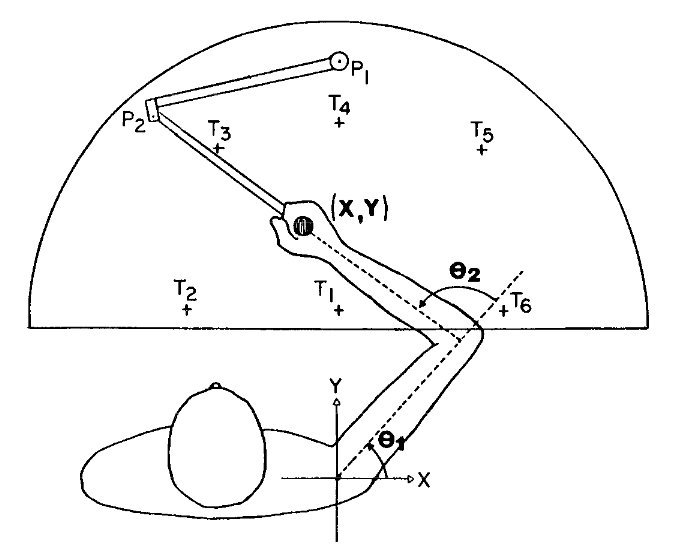
\includegraphics[width=0.4\textwidth]{./images/flashAndHoganExperiment.png}
			\end{center}
		\end{column}
	\end{columns}
\end{frame}

\begin{frame}[t]
	\frametitle{Motivation: Output of Motion Planners}
	\begin{itemize}
		\item Sampled based planners generated waypoints
	\end{itemize}
\end{frame}

\begin{frame}[fragile]
	\frametitle{Motivation: Current Classes Used in ROS Ecosystem}
	\begin{columns}
		\begin{column}{0.5\textwidth}
			\begin{itemize}
				\item Default ROS messages types for are defined as nested structrures.
				      The array-of-structures format leads to \emphImFusion{inefficient memory layout} and complicates the translation into the flat vector format that optimizers require.
				\item Other types are thighty coupled with the robot model
				\item do not provide clear interface for
				      \begin{itemize}
					      \item Evaluation at arbitrary time instantes
					      \item Computation of the derivatives
					      \item Time scaling
				      \end{itemize}
			\end{itemize}

		\end{column}
		\begin{column}{0.5\textwidth}
			Trajectory Message
			\begin{lstlisting}[basicstyle=\fontsize{5pt}{0pt}\selectfont\fontfamily{zi4}\selectfont]
std_msgs/msg/Header header
string[] joint_names
trajectory_msgs/msg/JointTrajectoryPoint[] points
            \end{lstlisting}
			Trajectory Point
			\begin{lstlisting}
double[] positions
double[] velocities
double[] accelerations
double[] effort
builtin_interfaces/msg/Duration time_from_start
                \end{lstlisting}
			Chomp trajectory
			\begin{lstlisting}
class ChompTrajectory
{
public:
...
    ChompTrajectory(const moveit::core::RobotModelConstPtr& robot_model, ...);
    double& operator()(size_t traj_point, size_t joint);
...
private:
...
    void init(); 
    std::string planning_group_name_;  
    Eigen::MatrixXd trajectory_;      
...
};
                \end{lstlisting}
		\end{column}
	\end{columns}
\end{frame}

\section{Goals}

\begin{frame}[t]
	\frametitle{Goals}

	{\fontsize{10}{5}
		\begin{itemize}
			\item Provide a unique interface to the user a \Verb|GSpline| class that represents all these minimum-X and more generic trajectories
			\item Design that class in terms of a minimal set of axioms derived from the mathematical foundations of the minimum-X optimization
			\item Expose the fundamental operations
			      \begin{itemize}
				      \item Derivatives
				      \item Elementary linear operations
				      \item Linear Scaling
				      \item Evaluate at arbitrary time instants
			      \end{itemize}
		\end{itemize}
	}
\end{frame}

\begin{frame}[t]
	\frametitle{Goals: Fundamental Axioms}
	{\fontsize{9}{5}
		\begin{itemize}
			\item defining Analytic operations (Analytical consistency)
			      \begin{equation*}
				      \diffk{}{t}{k}:\text{GSpline}\longrightarrow \text{GSpline}
			      \end{equation*}
			\item to define algebraic operations
			      \begin{eqnarray*}
				      +:\text{GSpline}\longrightarrow \text{GSpline}\\
				      \cdot:\mathbb{R} \times \text{GSpline}\longrightarrow \text{GSpline}
			      \end{eqnarray*}
			\item Linear Scaling
			      \begin{eqnarray*}
				      \left[t \rightarrow \sigma t \right]:\text{GSpline}\longrightarrow \text{GSpline}
			      \end{eqnarray*}
		\end{itemize}
		It's essential that these operations are closed within the same class: that is, performing any of these operations on instances of \Verb|GSpline| should result in another \Verb|GSpline| object
	}
\end{frame}
\begin{frame}[t]
	\frametitle{Goals: Monoid property}

	{\fontsize{10}{5}
		A \textbf{monoid} is an algebraic structure consisting of a set $M$ equipped with a binary operation
		$ \ast : M \times M \to M $ that satisfies the following properties:

		1. \textbf{Closure}:
		\begin{eqnarray*}
			\forall a, b \in M, \quad a \ast b \in M
		\end{eqnarray*}

		2. \textbf{Associativity}:
		\begin{eqnarray*}
			\forall a, b, c \in M, \quad (a \ast b) \ast c = a \ast (b \ast c)
		\end{eqnarray*}

		3. \textbf{Identity Element}:
		\begin{eqnarray*}
			\exists e \in M \text{ such that } \forall a \in M, \quad e \ast a = a \ast e = a
		\end{eqnarray*}

	}
\end{frame}
\begin{frame}[t]
	\frametitle{Goals: Monoid property}
	\begin{itemize}
		\item Composition is a fundamental tool in programming, the Monoid structure is the most fundamental compositional structure
	\end{itemize}

	
\includegraphics[height=0.2\textwidth]{./images/ccpconMonoids.png}
	
\includegraphics[height=0.2\textwidth]{./images/FunctionalProgrammingForDummies.jpeg}
\end{frame}


\section{Design}
\begin{frame}[t]
	\frametitle{Mathematical Foundations}

	We consider the problem of the minimization of a \emph{convex} combination of norms of the derivatives

	\begin{equation*}
		\min \int_{t_0}^{t_f} \alpha_1 \left\|\diff{\qv}{t}\right\|^2 + \alpha_2 \left\|\diffk{\qv}{t}{2}\right\|^2 + \cdots  + \alpha_1 \left\|\diffk{\qv}{t}{k} \right\|^2 \d t
	\end{equation*}

	And the corresponding Euler-Lagrange equations

	\begin{equation*}
		-\alpha_1 \diffk{\qv}{t}{2}+ \alpha_2 \diffk{\qv}{t}{4}- \cdots +  {(-1)}^k \alpha_k \diffk{\qv}{t}{2k}= 0 \ \ \text{a.e.}
	\end{equation*}

	At each time-interval we have
	\begin{equation*}
		\qv(t) = \xv_1 \basis_1
	\end{equation*}
\end{frame}

\begin{frame}[t]
	\frametitle{Mathematical Foundations: Features}

	We can prove that the solution of these ODEs respect the desired properites
		{\fontsize{10}{5}
			\begin{itemize}
				\item Analytical consistency:
				      \begin{equation*}
					      -\alpha_1 \diffk{}{t}{2} \left[\diff{\qv}{t}\right] +  \cdots +  {(-1)}^k \alpha_k \diffk{}{t}{2k} \left[\diff{\qv}{t}\right] = 0 \ \ \text{a.e.}
				      \end{equation*}
				\item Algebraic consistency I:\@ Linear Operations
				      \begin{eqnarray*}
					      -\alpha_1 \diffk{}{t}{2} \left[\qv_1 + \qv_2\right]  + \cdots +  {(-1)}^k \alpha_k \diffk{}{t}{2k} \left[\qv_1 + \qv_2\right] = 0 \ \ \text{a.e.}
				      \end{eqnarray*}
				\item Algebraic consistance II:\@ Linear Scaling
				      \only<1>{
					      \begin{eqnarray*}
						      -\alpha_1 \diffk{}{t}{2} \left[\qv(\sigma t)\right]  + \cdots +  {(-1)}^k \alpha_k \diffk{}{t}{2k} \left[\qv(\sigma t)\right] = 0 \ \ \text{a.e.}
					      \end{eqnarray*}
				      }
				      \only<2>{
					      \begin{eqnarray*}
						      -\warntext{\mathbf{\alpha}_1'} \diffk{}{t}{2} \left[\qv(\sigma t)\right]  + \cdots +  {(-1)}^k \alpha_k \diffk{}{t}{2k} \left[\qv(\sigma t)\right] = 0 \ \ \text{a.e.}
					      \end{eqnarray*}
				      }
			\end{itemize}
		}
\end{frame}
\begin{frame}[t]
	\frametitle{Mathematical Foundations: Linear Time-scaling invariance}
	If we desire a Time-scaling invariant cost function, we need to choose
	\begin{equation*}
		\min \int_{t_0}^{t_f} \frac{\alpha_1}{T^2} \left\|\diff{\qv}{t}\right\|^2 + \frac{\alpha_2}{T^4}\left\|\diffk{\qv}{t}{2}\right\|^2 + \cdots  + \frac{\alpha_k}{T^{2k}}\left\|\diffk{\qv}{t}{k} \right\|^2 \d t
	\end{equation*}
\end{frame}

\begin{frame}[fragile]
	\frametitle{Class Design: Overview}

	\begin{columns}
		\begin{column}{0.5\textwidth}
			\begin{lstlisting}[language=c++]
class GSpline {
private:
    Eigen::VectorXd time_interval_lengths_;
    Eigen::VectorXd coefficients_;
    double initial_time_;
    std::unique_ptr<Basis> basis_;
public:
    GSpline linear_scaling_new_execution_time(double _T) const;
    GSpline operator+(const GSpline& that);
    GSpline operator*(double num);
    GSpline derivative(std::size_t deg);
    bool operator()(double time) const;
};
    \end{lstlisting}
		\end{column}
		\begin{column}{0.5\textwidth}
			\begin{lstlisting}[language=C++]
class Basis {
protected:
    Eigen::VectorXd parameters_float_;
    Eigen::VectorXi parameters_int_;
public:
    virtual void eval_on_window(
                    ..., Eigen::VectorXd&_buff) const = 0;
    virtual void eval_derivative_on_window(
                    ..., Eigen::VectorXd& _buff) const = 0;
    virtual void eval_derivative_wrt_tau_on_window(
                    ..., Eigen::VectorXd& _buff) const = 0;

    virtual std::unique_ptr<Basis> clone() const = 0;
};
    \end{lstlisting}
		\end{column}
	\end{columns}
	\begin{center}
		\begin{tikzpicture}[scale=0.9]
			\tikzumlset{font=\fontsize{5}{4}\selectfont}
			\umlemptyclass{GSpline}
			\umlemptyclass[x=7, y=0]{Basis}
			\umlunicompo [angle1=-90, angle2=-140 ] {GSpline}{Basis}
			\umlemptyclass[x=3, y=-2]{BasisLagrange}
			\umlemptyclass[x=6, y=-2]{BasisLegendre}
			\umlemptyclass[x=9, y=-2]{CustomBasis}
			\umlVHVinherit[] {CustomBasis}{Basis}
			\umlVHVinherit[] {BasisLagrange}{Basis}
			\umlVHVinherit[] {BasisLegendre}{Basis}
		\end{tikzpicture}
	\end{center}
\end{frame}

\begin{frame}[fragile]
	\begin{itemize}
		\item Polynomial Basis solution of
		      \begin{eqnarray}
			      \min \int_{t_0}^{t_f} \left\|\diffk{\qv}{t}{k}\right\|^2 \d t
		      \end{eqnarray}
		      \begin{itemize}
			      \item  \Verb|basis::BasisLegendre|
			      \item  \Verb|basis::BasisLagrange|
		      \end{itemize}
		\item Non Polynomial basis
		      \begin{eqnarray}
			      \min \int_{t_0}^{t_f} \alpha \left\|\diffk{\qv}{t}{}\right\|^2  + (\alpha - 1 )\left\|\diffk{\qv}{t}{3}\right\|^2 \d t
		      \end{eqnarray}
		      \begin{itemize}
			      \item  \Verb|basis::Basis0101|
		      \end{itemize}
	\end{itemize}
\end{frame}

\begin{frame}[fragile]
	\frametitle{Design: General operations}
	We also desire to work with trajectories that are not gsplines
	\begin{itemize}
		\item The norm of a derivative ${\left\| \ddot \qv \right\|}^2$
		\item Non linear parametrization $ \qv \circ s $, where $\qv, s\in \text{\Verb|GSpline|}$
	\end{itemize}
	For this reason we also provide interface to construct expressions
	\begin{itemize}
		\item Addition and scalar multiplication
		\item Concatenating functions
		\item Compisition
	\end{itemize}
	\begin{center}
		\begin{tikzpicture}[scale=0.9]
			\tikzumlset{font=\fontsize{5}{4}\selectfont}
			\umlemptyclass[x=0, y=0]{FunctionBase}
			\umlemptyclass[x=-3, y=-2]{CustomFunction}
			\umlemptyclass[x=3, y=-2]{FunctionExpression}
			\umlVHVinherit[] {FunctionExpression}{FunctionBase}
			\umlVHVinherit[] {CustomFunction}{FunctionBase}
			\umlHVHunicompo[anchor1=east,angle1=0, arm1=1cm, angle2=0,mult1=1, mult2=1..*] {FunctionExpression}{FunctionBase}
		\end{tikzpicture}
	\end{center}
\end{frame}
\begin{frame}[fragile]
	\frametitle{Design: General Overview}
	\begin{center}
		\begin{tikzpicture}
			\tikzumlset{font=\fontsize{5}{4}\selectfont}
			\umlemptyclass[x=0, y=0]{FunctionBase}
			\umlemptyclass[x=3, y=-2]{FunctionExpression}
			\umlVHVinherit[] {FunctionExpression}{FunctionBase}
			\umlHVHunicompo[anchor1=east,angle1=0, arm1=1cm, angle2=0,mult1=1, mult2=1..*] {FunctionExpression}{FunctionBase}
			\tikzumlset{font=\fontsize{5}{4}\selectfont}
			\umlemptyclass[y=-4]{GSpline}
			\umlemptyclass[x=7, y=-4]{Basis}
			\umlunicompo [angle1=-90, angle2=-140 ] {GSpline}{Basis}
			\umlemptyclass[x=3, y=-6]{BasisLagrange}
			\umlemptyclass[x=6, y=-6]{BasisLegendre}
			\umlemptyclass[x=9, y=-6]{CustomBasis}
			\umlVHVinherit[] {CustomBasis}{Basis}
			\umlVHVinherit[] {BasisLagrange}{Basis}
			\umlVHVinherit[] {BasisLegendre}{Basis}
			\umlVHVinherit[] {GSpline}{FunctionBase}
		\end{tikzpicture}
	\end{center}
\end{frame}


\begin{frame}[t]
	\frametitle{Optimization: Dependices}

	For optimization we rely on
	\begin{itemize}
		\item 
\includegraphics[height=1cm]{images/ifopt.png}
		\item 
\includegraphics[height=2cm]{images/Ipopt.png}
	\end{itemize}
\end{frame}

\begin{frame}[t]
	\frametitle{Optimization: Interface}

	We provide out-of-the-box optimiuation
	\begin{itemize}
		\item trajectory optimization
		\item Minium time path-consisten stop
	\end{itemize}
\end{frame}

\begin{frame}[fragile]
	\frametitle{OpStop}
\end{frame}

\begin{frame}[fragile]
	\frametitle{Integration with ROS types}
	\begin{lstlisting}
        #  This message represents a generalized spline
        # Name of the basis
        string name
        # Dimension of the vector space defined by the basis
        int32 dim
        # Parameters
        float64[] parameters
	\end{lstlisting}
	\begin{lstlisting}
        #  This message represents a generalized spline

        float64 domain_left_boundary
        float64 domain_right_boundary
        int32 codom_dim
        int32 number_of_intervals
        gsplines_msgs/Basis basis
        float64[] coefficients
        float64[] interval_lengths
	\end{lstlisting}
	\begin{lstlisting}
        Header header
        string[] name
        gsplines_msgs/GSpline gspline
	\end{lstlisting}
	\begin{itemize}
		\item \Verb|trajectory_msgs::JointTrajectory|
		\item \Verb|control_msgs::FollowJointTrajectoryGoal|

	\end{itemize}
\end{frame}

\begin{frame}[fragile]
	\frametitle{Integration with ROS Control}
	\begin{itemize}
		\item \Verb|FollowJointGSpline.action|
	\end{itemize}

	\begin{center}
		\begin{tikzpicture}
			\tikzumlset{font=\fontsize{5}{4}\selectfont}
			\umlbasiccomponent[x=0, y=-3]{ROSAPP}
			\umlbasiccomponent[x=4]{ActionWrapper}
			\umlbasiccomponent[x=7,y=-3]{ROSControl}
			\umlVHassemblyconnector[interface=FollowJointGSplineAction ,first arm, anchor2=-160] {ROSAPP}{ActionWrapper}
			\umlVHassemblyconnector[interface=FollowJointTrajectoryAction ,first arm, anchor2=0] {ROSControl}{ActionWrapper}
		\end{tikzpicture}
	\end{center}

\end{frame}

\begin{frame}[t]
	\frametitle{OpStop Integration}
	\begin{center}
		\begin{tikzpicture}
			\tikzumlset{font=\fontsize{5}{4}\selectfont}
			\umlbasiccomponent[x=0, y=-3]{ROSAPP}
			\umlbasiccomponent[x=4]{ActionWrapper}
			\umlbasiccomponent[x=7,y=-3]{ROSControl}
			\umlVHassemblyconnector[interface=FollowJointGSplineAction ,first arm, anchor2=-160] {ROSAPP}{ActionWrapper}
			\umlVHassemblyconnector[interface=FollowJointTrajectoryAction ,first arm, anchor2=0] {ROSControl}{ActionWrapper}
		\end{tikzpicture}
	\end{center}
\end{frame}

\begin{frame}[t]
	\frametitle{OpStop Integration}
	\begin{center}
		\begin{tikzpicture}
			\begin{umlseqdiag}
				\tikzumlset{font=\fontsize{5}{4}\selectfont}
				\umlobject{ROSAPP}
				\umlobject{ActionWrapper}
				\umlobject{ROSControl}
				\begin{umlcall}[op=FollowJointGSplineGoal,return=FollowJointGSplineFeedBack]{ROSAPP}{ActionWrapper}
					\begin{umlcall}[op=FollowJointGSplineGoal,return=FollowJointTrajectoryFeedBack]{ActionWrapper}{ROSControl}
					\end{umlcall}
				\end{umlcall}
				\begin{umlcall}[op=FollowJointGSplineCancel]{ROSAPP}{ActionWrapper}
					\begin{umlcallself}[op=optimization]{ActionWrapper}{ActionWrapper}
					\end{umlcallself}
					\begin{umlcall}[op=FollowJointGSplineGoal,return=FollowJointTrajectoryFeedBack]{ActionWrapper}{ROSControl}
					\end{umlcall}
				\end{umlcall}
			\end{umlseqdiag}
		\end{tikzpicture}
	\end{center}
\end{frame}

\begin{frame}[fragile]
	\frametitle{Integration with Moveit}
	\begin{itemize}
		\item Planner adapter \Verb|gsplines_moveit/MinimumSobolevSeminormAdapter|, can be used inside \Verb|ompl| pipeline
		      \begin{lstlisting}
gsplines_moveit/MinimumSobolevSeminormAdapter
default_planner_request_adapters/FixWorkspaceBounds
default_planner_request_adapters/FixStartStateBounds
default_planner_request_adapters/FixStartStateCollision
default_planner_request_adapters/FixStartStatePathConstraints
	          \end{lstlisting}
		\item  Controller Manager \Verb|gsplines_moveit/GSplinesControllerManager|
	\end{itemize}
\end{frame}

\begin{frame}[t]
	\frametitle{Integration with Moveit}

\end{frame}

\end{document}
